\section{Datos}

Ya que en el montaje, el termómetro medía directamente la temperatura
de la varilla, no hace falta referirnos a las primeras ecuaciones, las
cuales nos sirvieron para ilustrar cómo el circuito iba a generar calor
en la varilla.

La temperatura inicial, o de ambiente, medida fue $T_0 =\qty{20.3}{\degreeCelsius}$.
La longitud inicial medida fue $L_0 = \qty{68.3}{\cm}$.
\begin{center}
  \begin{tabular}{|>{$}c<{$}| >{$}c<{$}| >{$}c<{$}|}
    \hline
    \text{Temperatura}(\si{\degreeCelsius}) & \Updelta L(\si{\micro\m})  & \Updelta T\\
    \hline
    20.8  & 10  & 0.5\\
    22.7  & 1.5 & 2.4\\
    21.7  & 4   & 1.4\\
    26.7  & 12  & 6.4\\
    36.5  & 24  & 16.2\\
    41.2  & 32  & 20.9\\
    45.0  & 40  & 24.7\\
    54.0  & 51  & 33.7\\
    \hline
  \end{tabular}
\end{center}

La linealización es entonces:
\begin{center}
  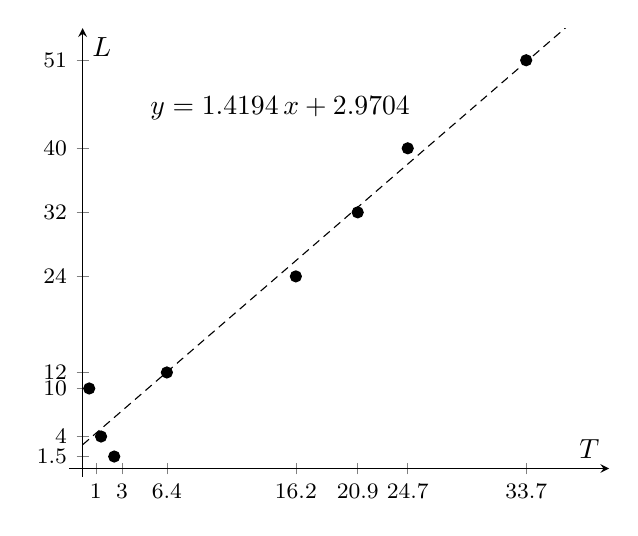
\begin{tikzpicture}
    \begin{axis}[
      xmin=-1,
      xmax=40,
      ymin=-1,
      ymax=55,
      xlabel=$\Updelta T$,
      ylabel=$\Updelta L$,
      xtick={1,3,6.4,16.2,20.9,24.7,33.7},
      ytick={10,1.5,4,12,24,32,40,51},
      axis lines=center,
      enlarge x limits=0.00001,
      enlarge y limits=0.00001,
      tick label style={font=\footnotesize}
    ]
    \addplot[
      only marks,
      ]
      table[x=x,y=y]{
        x   y
        0.5		10
        2.4		1.5
        1.4		4
        6.4		12
        16.2	24
        20.9	32
        24.7	40
        33.7	51
      };

      \addplot[
        densely dashed,
        domain=0:40,
      ]{
        1.4194*x + 2.9704
      };

      \node at (15,45) {$y = 1.4194\,x + 2.9704$};
    \end{axis}
  \end{tikzpicture}
\end{center}

Una vez con esta linealización, para que las unidades en el cálculo tengan
sentido, hace falta tomar $L_0$ en \si{\micro\m}. Así, el valor obtenido es:
\[\upalpha = \frac{1.4194}{L_0} = 
\frac{1.4194}{\qty{68.3e3}{\micro\m}} = 
\qty[per-mode=reciprocal]{2.07818e-5}{\per\degreeCelsius}\]

De este dato, viendo los coeficientes en una tabla para diferentes elementos, se encontró
que los más aproximados eran el de la plata (\qty[per-mode=reciprocal]{2.0e-5}{\per\degreeCelsius})
y el del aluminio (\qty[per-mode=reciprocal]{2.4e-5}{\per\degreeCelsius})